%=========================
\chapter{La liste chainée}
%=========================

\begin{center}
	\href{http://static.commentcamarche.net/www.commentcamarche.net/faq/images/0-Anm7iJKj-dl-ex2-s-.png}
	{\includegraphics[width=6.094cm,height=4.094cm]{image/listechainee.png}}
\end{center}

	\marginicon{objectif}
	Tout comme un tableau, une liste chainée est une collection d'éléments. 
	Mais, contrairement aux tableaux, les éléments ne sont pas contigus 
	en mémoire mais «~chainés~». Nous voyons ses avantages et inconvénients 
	par rapport aux tableaux, comment les implémenter en orienté-objet 
	et en non orienté-objet et les opérations de base sur les listes.


%=====================
\section{Définitions}
%=====================


	Voici quelques définitions de la liste chainée (\textit{linked list} 
	en anglais) issues de différents livres sur le
	sujet. Elles nous indiquent à la fois à quoi cela ressemble 
	et l'utilité d'une telle structure.
	
	\begin{itemize}
		\item 
			\textit{Une liste chainée désigne en informatique une structure de données
			représentant une collection ordonnée et de taille arbitraire d'éléments 
			de même type. L'accès aux éléments d'une liste se fait de manière 
			séquentielle~: chaque élément permet l'accès au suivant, 
			contrairement au cas du tableau dans lequel l'accès se fait de
			manière absolue, par adressage direct de chaque cellule 
			du dit tableau.} 
			(Wikipédia, août 2013)
		\item
			\textit{Une liste est un conteneur séquentiel capable d'insérer 
			et de supprimer des éléments localement de façon constante, 
			c'est-à-dire indépendamment de la taille du conteneur.} 
			(Structures de données en Java -- Hubbard -- ed. Schaum's)
	\item
		\textit{Les listes sont des conteneurs destinés aux insertions 
		s'effectuant en temps constant quelle que soit la position 
		dans le conteneur.} 
		(La bibliothèque standard STL du C++ -- Fontaine -- InterEditions)
	\item
		\textit{Une liste chainée est une structure de données dans 
		laquelle les objets sont arrangés linéairement. Toutefois,
		contrairement au tableau, pour lequel l'ordre linéaire est 
		déterminé par les indices, l'ordre d'une liste chainée est
		déterminé par un pointeur dans chaque objet.} 
		(Introduction à l'algorithmique -- Cormen, Leiserson, Rivest -- Dunod)
\end{itemize}


%===================================
\section{Liste versus liste chainée}
%===================================

	Dans la terminologie moderne, le terme \textit{liste} est 
	plutôt utilisé pour dénoter toute collection séquentielle
	d'éléments (il existe un premier élément, un deuxième, ...). 
	Autrement dit, chaque élément a une position précise dans
	la collection. En ce sens, un tableau ou un fichier sont 
	également des \textit{listes} !
	
	On peut opposer la liste à la structure d'\textit{ensemble} 
	où les éléments ne sont pas positionnés (un élément
	\textit{est} ou \textit{n'est pas} dans un ensemble mais 
	sans que sa position puisse être donnée).
	
	Le concept de liste ne doit pas être confondu avec la notion 
	de \textit{tri}. On peut parler de la \textit{liste}
	contenant les éléments 3, 8 et 2 dans cet ordre 
	(au sens de \textit{séquence} et pas d'\textit{ordre de tri}).


%=======================================
\section{Représentation et terminologie}
%=======================================

	Pour écrire explicitement une liste chainée et son contenu 
	sous forme compacte, on indique la liste des valeurs qu'elle
	contient entre parenthèses. Exemple~: la liste (3, 6, 5, 2).
	
	Schématiquement, on la représente plutôt ainsi~:

	\begin{center}
	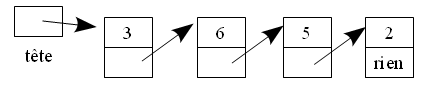
\includegraphics[width=11.324cm,height=2.355cm]{image/a2012Logique2eme-img002.png}
	\end{center}
	
	De ce schéma, il apparait que chaque \textbf{élément} 
	d'une liste chainée est composé de 2 parties~: la valeur
	proprement dite et un \textit{accès} à l'élément suivant. 
	De plus, on accède au premier élément de la liste via une
	zone spéciale, la \textbf{tête} de la liste chainée.

	Le dernier élément n'ayant pas de suivant, on indique \textit{rien} 
	dans la zone réservée à l'accès au suivant. Dans la
	littérature et selon les langages, on trouvera, à la place de \textit{rien}, 
	les notations \textit{null}, \textit{nil}, ... ou encore Ø.
	
	Le schéma ci-dessus peut encore se compactifier davantage, 
	en une forme qui ne fait pas apparaitre la tête de liste ni
	les accès aux éléments suivants~:

	\begin{center}
	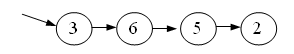
\includegraphics[width=7.779cm,height=1.429cm]{image/a2012Logique2eme-img003.png}
	\end{center}
	
	Au contraire du tableau, donc, il n'y a pas d'accès direct à un élément 
	(en donnant son indice) mais il est nécessaire
	de partir du premier élément et de suivre la «~\textit{chaine~»}. 
	Comment représenter ce \textit{lien}, cet
	\textit{accès} en mémoire ? Cela dépend du type de langage~:

	\begin{itemize}
		\item
			en programmation procédurale (non orienté-objet), 
			on utilise la notion de pointeur (cf. le cours de C/C++) tout en
			montrant qu'il est même possible de s'en sortir avec un langage 
			qui ne dispose pas de la notion de pointeur (comme par exemple Cobol) ;
		\item
			en orienté-objet (OO), un élément est représenté par un objet 
			dont un attribut est une référence vers l'objet
			représentant l'élément suivant.
	\end{itemize}


%===========================================================
\section{Rappel~: opérations sur les tableaux et complexité}
%===========================================================

	Afin de mieux comprendre ce qu'apporte la liste chainée 
	par rapport au tableau, revoyons ce que «~coûte~» les opérations
	courantes sur les tableaux. Le tableau ci-dessous donne la complexité 
	(par l'algorithme le plus économique) des
	opérations élémentaires pour un tableau trié et non trié.

	\begin{center}
		\tablefirsthead{}
		\tablehead{}
		\tabletail{}
		\tablelasttail{}
		\begin{supertabular}{|m{5.511cm}|m{3.6139998cm}|m{3.631cm}|}
		\hline
		\bfseries Opération &
		\bfseries Tableau non trié &
		\bfseries Tableau trié\\
		\hline
		Ajout d'un élément &
		\centering{O(1)} &
		\centering\arraybslash{O($n$)}\\
		\hline
		{Suppression d'un élément} &
		\centering{O($n$)} &
		\centering\arraybslash{O($n$)}\\
		\hline
		{Recherche d'un élément} &
		\centering{O($n$)} &
		\centering\arraybslash{O($log_{2}n$)}\\
		\hline
		{Parcours} &
		\centering{O($n$)} &
		\centering\arraybslash{O($n$)}\\\hline
		\end{supertabular}
	\end{center}
	
	Pour rappel, la notation O($n$) indique que l'opération 
	prend un temps qui est proportionnel à $n$, la
	taille du tableau. La plupart des opérations sont de complexité 
	O($n$), par exemple, lors d'une suppression, il
	faut décaler des éléments pour boucher le trou qui est apparu. 
	Il en est de même pour un ajout dans un tableau trié. Si
	le tableau n'est pas trié, il est évident qu'on peut rajouter 
	l'élément en fin de tableau, ce qui est immédiat
	(complexité O(1)). Dans le cas d'un tableau trié, c'est 
	l'algorithme de recherche dichotomique qui permet de trouver
	rapidement un élément avec une complexité O($log_{2}n$).

%==================================================
\section{Ajout d'un élément dans une liste chainée}
%================================================== 

	Dans une liste chainée (qu'elle soit ordonnée ou non), 
	il n'est pas nécessaire de décaler des éléments pour un ajouter
	un. Reprenons la liste chainée de l'exemple ci-dessus 
	et ajoutons l'élément 8 entre le 6 et le 5~:

	\ Avant~: \ \ \ \ \ \ \ \ \ \ \ \ \ \ \ \ \ \ \ \ \ \ \ \ \ \ \ \ \ \ \ \ \ \ \ \ \ \ \ \ \ \ \ \ \ \ \ \ \ \ \ \ \ \ \ \ \ \ Après~:

	 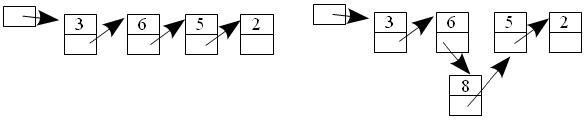
\includegraphics[width=15.558cm,height=3.334cm]{image/a2012Logique2eme-img004.png} 

	Il aura suffi de modifier des «~flèches~» (c'est-à-dire des «~liens~» 
	ou des «~accès~»). L'opération prend donc le même
	temps quelle que soit la taille de la liste chainée 
	(pour autant qu'on soit déjà positionné à l'endroit de l'ajout).

	La complexité de cette opération est donc O(1). Il n'y a ici pas de décalage d'éléments comme pour un tableau, pour la
	simple raison que les éléments d'une liste chainée n'ont aucune raison d'être à des endroits contigus dans la mémoire
	de l'ordinateur.

	Il y a un ajout qui fait figure de cas particulier, c'est l'ajout en tête de liste chainée, car il modifie
	obligatoirement l'accès au premier élément. Par exemple, si nous ajoutons 8 en première position, cela donne~:

	\ Avant~: \ \ \ \ \ \ \ \ \ \ \ \ \ \ \ \ \ \ \ \ \ \ \ \ \ \ \ \ \ \ \ \ \ \ \ \ \ \ \ \ \ \ \ \ \ \ \ \ \ \ \ \ \ \ \ \ \ \ Après~:

	 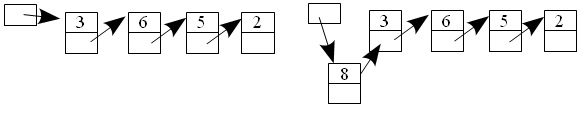
\includegraphics[width=15.452cm,height=3.122cm]{image/a2012Logique2eme-img005.png}
	
	
%========================================================
\section{Suppression d'un élément dans une liste chainée}
%========================================================
	
	La suppression d'un élément se fait tout aussi simplement. 
	L'opération est également de complexité O(1). Par exemple,
	supprimons l'élément de valeur 6~: 
	
	
	\ Avant~: \ \ \ \ \ \ \ \ \ \ \ \ \ \ \ \ \ \ \ \ \ \ \ \ \ \ \ \ \ \ \ \ \ \ \ \ \ \ \ \ \ \ \ \ \ \ \ \ \ \ \ \ \ \ \ \ \ \ Après~:

	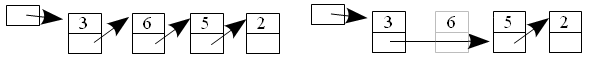
\includegraphics[width=15.61cm,height=1.773cm]{image/a2012Logique2eme-img006.png} 

	Ici aussi, le cas de la suppression du premier élément est particulier~:

	\ Avant~: \ \ \ \ \ \ \ \ \ \ \ \ \ \ \ \ \ \ \ \ \ \ \ \ \ \ \ \ \ \ \ \ \ \ \ \ \ \ \ \ \ \ \ \ \ \ \ \ \ \ \ \ \ \ \ \ \ \ Après~:

	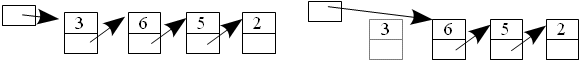
\includegraphics[width=15.425cm,height=1.72cm]{image/a2012Logique2eme-img007.png} 

	Remarquez que l'élément, quoique supprimé de la liste chainée, 
	est encore présent sur les schémas. Bien que l'élément ne
	fasse plus logiquement partie de l'ensemble des éléments 
	de la liste chainée, il est encore présent physiquement dans
	la mémoire. La suppression définitive de l'élément est gérée 
	soit par le programmeur lui-même, soit c'est le système
	qui nettoie de la mémoire les éléments auxquels plus aucun accès ne mène. 
	C'est le rôle du \textit{garbage collector},
	solution que nous avons adoptée en logique OO, 
	mais qui n'est pas vraie pour tous les langages OO (cf. C++).



%===============================
\section{Recherche d'un élément}
%===============================

	La recherche d'un élément dans une liste chainée non triée 
	est similaire à celle d'un tableau, il faut obligatoirement
	tout parcourir pour savoir si l'élément est présent ou non.

	Au contraire d'un tableau, le fait de savoir que la liste chainée 
	est triée (sur les valeurs des éléments) ne permet pas
	de développer un algorithme rapide de type \textit{recherche dichotomique}. 
	Tout au plus on peut, comme avec un tableau, s'arrêter lorsqu'on 
	dépasse la position où l'élément recherché aurait dû se trouver.


%=====================================
\section{Liste chainée versus tableau}
%=====================================

	Rajoutons dans le tableau ce que l'on a vu 
	de la complexité des listes chainées~:

	\begin{center}
		\tablefirsthead{}
		\tablehead{}
		\tabletail{}
		\tablelasttail{}
		\begin{supertabular}{|m{5.145cm}|m{2.023cm}|m{1.7329999cm}|m{2.836cm}|m{2.675cm}|}
		\hline
		{\bfseries Opération} &
		{\bfseries Tableau non trié} &
		{\bfseries Tableau trié} &
		{\bfseries Liste chainée non triée} &
		{\bfseries Liste chainée triée}\\
		\hline
		{Ajout d'un élément} &
		\centering{O(1)} &
		\centering{O($n$)} &
		\centering{O(1)} &
		\centering\arraybslash{O(1)}\\
		\hline
		{Suppression d'un élément} &
		\centering{O($n$)} &
		\centering{O($n$)} &
		\centering{O(1)} &
		\centering\arraybslash{O(1)}\\
		\hline
		{Recherche d'un élément} &
		\centering{O($n$)} &
		\centering{O($log_{2}n$)} &
		\centering{O($n$)} &
		\centering\arraybslash{ O($n$)}\\
		\hline
		{Parcours} &
		\centering{O($n$)} &
		\centering{O($n$)} &
		\centering{O($n$)} &
		\centering\arraybslash{O($n$)}\\
		\hline
		\end{supertabular}
	\end{center}
	
	On voit que la liste chainée montre tout son intérêt pour les ajouts 
	et les suppressions mais se montre moins efficace
	pour les recherches dans le cas où l'information est triée.

	Le choix d'un tableau ou d'une liste chainée pour représenter 
	une collection dans un problème précis dépend dès lors du
	rapport entre le nombre d'ajouts/suppressions et de recherches 
	que l'on compte effectuer.

	
	Remarquons aussi que dans le cas où les ajouts/suppressions se font 
	en \textit{fin} de tableau (le cas d'une \textit{pile} par exemple), 
	la complexité rejoint celle d'une liste chainée.

	Nous allons étudier l'implémentation de la liste chainée, 
	d'abord procédurale (ou \textit{«~C-like~»}) car c'est celle
	que vous utiliserez au labo C, ensuite nous verrons l'implémentation OO.


%===================================
\section{Implémentation procédurale}
%===================================

	\subsection{Notations}
	%=====================
	
	Pour les besoins de cette implémentation, nous devons introduire 
	une nouvelle notation~: l'\textbf{accès} à une
	variable, ou encore \textbf{référence} ou \textbf{pointeur}.

	La déclaration de cet accès ce fera comme suit~:

	\cadre{
		\begin{pseudo}
			\Decl p~: accès à T
		\end{pseudo}
	}

	ce qui signifie que \textstyleCodeInsr{p} permet d'accéder à un élément 
	de type \textstyleCodeInsr{T}. 
	Dans le cadre de ce cours, comme les éléments d'une liste
	chainée peuvent être vus comme composés (structurés) d'un champ valeur 
	et d'un champ accès, nous n'aurons que des accès
	à des structures mais les langages non objets permettent généralement 
	des accès vers des éléments de type quelconque.

	Dans le contexte des références, il faut pouvoir créer dynamiquement 
	l'élément référencé. Cela s'indique par la
	primitive \textstyleCodeInsr{allouer}, à utiliser comme suit~:

	\cadre{
		\begin{pseudo}
			\Decl p \Gets \Alloc(T)
		\end{pseudo}
	}
	
	où \textstyleCodeInsr{T} est le type de l'élément référencé. 

	\textbf{Exemple}~: 
	\begin{pseudo}
		\Decl p \Gets \Alloc(Personne)
	\end{pseudo}
	
	Cette instruction provoque l'allocation d'un espace mémoire pour
	une variable de type \textstyleCodeInsr{Personne} et l'accès à 
	cet espace est placé dans \textstyleCodeInsr{p}. 
	En C, p pourrait être un pointeur recevant
	l'adresse de l'espace alloué lors de cette demande d'allocation.

	Pour accéder à la variable d'accès \textstyleCodeInsr{p}, 
	on utilisera la flèche vers la droite (comme en C), et donc,
	\cadre{
		\begin{pseudo}
			\Stmt p\Gives truc
		\end{pseudo}
	}
	
	désignera le champ \textit{truc} de la variable accessible par \textstyleCodeInsr{p}.

	
	Pour récupérer l'espace mémoire inutilement occupé par une variable 
	qui n'est plus utilisée, on a l'opération inverse
	qui se notera par la nouvelle primitive~:

	\cadre{
		\begin{pseudo}
			\Free p
		\end{pseudo}
	}
	
	qui supprime définitivement la variable d'accès \textstyleCodeInsr{p}, 
	ce qui a pour effet de rendre cet espace mémoire à nouveau
	allouable.

	Nous avons vu qu'un élément de liste est composé d'un champ \textit{valeur} 
	(qui contient la valeur proprement dite de
	l'élément) et d'un champ permettant d'accéder à l'élément suivant, 
	que nous nommerons simplement \textit{suivant}. Le
	type \textstyleCodeInsr{T} de la valeur de l'élément est noté entre crochets~:
	
	\cadre{
		\begin{pseudo}
			\Struct{ÉlémentListe<T>}
				\Decl valeur~: T
				\Decl suivant~: accès à ÉlémentListe<T>
			\EndStruct
		\end{pseudo}
	}
	
	\textbf{Exemple}~: pour un élément de liste chainée d'entiers, on définirait la structure~:
	
	\cadre{
		\begin{pseudo}
			\Struct{ÉlémentListe<entier>}
				\Decl valeur~: entier
				\Decl suivant~: accès à ÉlémentListe<entier>
			\EndStruct
		\end{pseudo}
	}
	
	En non orienté-objet, une liste chainée se reconnait simplement 
	par le fait que des éléments semblables (de même type)
	sont chainés, ce qui signifie que chacun d'eux contient un accès 
	à son suivant. Pour manipuler un tel ensemble de
	données, la seule condition est de pouvoir accéder au premier 
	élément de cet ensemble par une variable de type \textstyleCodeInsr{accès},
	que l'on peut appeler \textit{premier}, \textit{têteListe} ou encore 
	\textit{TL} (et qui n'a nul besoin d'être
	structurée). La liste chainée n'est donc rien d'autre qu'un accès, 
	celui au premier élément. Si cette liste est vide,
	cet accès a pour valeur \textit{rien}~:

	\cadre{
		\begin{pseudo}
			\Decl têteListe~: accès à ÉlémentListe<T> 
			\RComment accès au premier élément, rien si vide
		\end{pseudo}
	}

	\textbf{Exemple}~: pour déclarer une liste chainée d'entiers, on aurait~:

	\cadre{
		\begin{pseudo}
			\Decl têteListe~: accès à ÉlémentListe<entier>
		\end{pseudo}
	}

	\subsection{Exemple~1~: taille d'une liste chainée}
	%==================================================
	
		Voici un exemple d'algorithme calculant le nombre 
		d'éléments d'une liste chainée d'accès TL.
		
		\cadre{
			\begin{pseudo}
				\Module{tailleListeChainée}{TL~: accès à ÉlémentListe<T>}{entier}
					\Decl courant~: accès à ÉlémentListe<T>
					\Decl cpt~: entier
					\Let cpt \Gets 0
					\Let courant \Gets TL
					\While{courant ${\neq}$ rien}
						\Let cpt \Gets cpt + 1
						\Let courant \Gets courant\Gives suivant
					\EndWhile
					\Return cpt
				\EndModule
			\end{pseudo}
		}
			
	\subsection{Exemple~2~: mise d'un fichier en liste chainée}
	%==========================================================
		
		Dans ce 2\textsuperscript{ème} exemple, on montre comment mettre 
		le contenu d'un fichier de variables structurées
		Identité (nom, prénom~: chaines, dateNais~: Date) dans une liste chainée.
		
		\cadre{
			\begin{pseudo}
				\Module{miseEnListe}{Personnes~: fichier de Identité}{accès à ÉlémentListe<Identité>}
					\Decl courant, précédent, TL~: accès à ÉlémentListe<Identité>
					\Decl enr~: Identité
					\Let TL \Gets rien 
					\RComment la liste est vide au départ
					\Stmt \K{ouvrir} Personne (\K{IN})
					\Read Personnes ; enr
					\If{NON EOF(Personnes)}
					\RComment traitement spécial pour le 1\textsuperscript{er} enregistrement
						\Decl TL \Gets \Alloc(ÉlémentListe<Identité>)
						\Decl TL\Gives valeur \Gets enr
						\Decl TL\Gives suivant \Gets rien
						\Decl précédent \Gets TL
						\Read Personnes ; enr
					\EndIf
					\While{NON EOF(Personnes)}
						\Decl courant \Gets \Alloc(ÉlémentListe<Identité>)
						\Decl courant\Gives valeur \Gets enr
						\Decl courant\Gives suivant \Gets rien
						\Decl précédent\Gives suivant \Gets courant
						\Decl précédent \Gets courant
						\Read Personnes ; enr
					\EndWhile
					
					\Stmt \K{fermer} Personnes
					\Return TL
				\EndModule
			\end{pseudo}
		}
		
		
%=====================================
\section{Représentation sans pointeur}
%=====================================

	La plupart des langages non orienté-objet possèdent la notion 
	de pointeur mais il y a des exceptions (Cobol par
	exemple). Comment implémenter une liste chainée dans un tel langage? 
	En simulant par exemple la liste chainée via un
	tableau qui contient 2 champs (la valeur de l'élément 
	et l'indice de l'élément suivant).

	\textbf{Exemple}~: la liste chainée (3, 6, 5, 2) 
	pourrait être donnée par le tableau suivant~:

	\begin{center}
		\tablefirsthead{}
		\tablehead{}
		\tabletail{}
		\tablelasttail{}
		\begin{supertabular}{|m{0.40900004cm}|m{0.403cm}|m{0.403cm}|m{0.403cm}|m{0.38200003cm}|}
		\multicolumn{1}{m{0.40900004cm}}{{\itshape 1}} &
		\multicolumn{1}{m{0.403cm}}{{\itshape 2}} &
		\multicolumn{1}{m{0.403cm}}{{\itshape 3}} &
		\multicolumn{1}{m{0.403cm}}{{\itshape 4}} &
		\multicolumn{1}{m{0.38200003cm}}{{\itshape 5}}\\\hline
		{ 2} &
		{ 6} &
		{ 3} &
		{ 5} &
		{ ?}\\
		\hline
		{ 0} &
		{ 4} &
		{ 2} &
		{ 1} &
		{ ?}\\
		\hline
		\end{supertabular}
	\end{center}

	À condition de savoir aussi où commencer, c'est-à-dire connaitre 
	l'indice du premier élément (le 3\textsuperscript{ème}
	dans notre exemple). L'indice 0 indique la fin de la liste chainée. 
	Pour ajouter un élément, il suffit de l'ajouter en
	fin de tableau et d'adapter les indices sur la deuxième ligne. 
	La suppression est aussi aisée mais crée un «~trou~»
	qu'il faut pouvoir gérer (par exemple via une liste des places libres). 


%=====================================
\section{Implémentation orienté-objet}
%=====================================

	\subsection{implémentation}
	%==========================
		
		Pour l'implémentation OO, nous allons définir deux classes, 
		une pour un élément de liste chainée, et une autre pour la
		liste chainée elle-même.

		\cadre{
			\begin{pseudo}
				\Class{ÉlémentListe<T>}
					\Private
						\Decl valeur~: T
						\Decl suivant~: ÉlémentListe<T>
					\Public
						\ConstrSign{ÉlémentListe<T>}{val~: T, elt~: ÉlémentListe<T>}
						\ConstrSign{ÉlémentListe<T>}{val~: T}
						\RComment suivant à rien
						\MethodSign{getvaleur}{}{T}
						\MethodSign{setValeur}{val~: T}{}
						\MethodSign{getSuivant}{}{ÉlémentListe<T>}
						\RComment ne renvoie rien si pas de suivant
						\MethodSign{setSuivant}{elt~: ÉlémentListe<T>}{}
				\EndClass
			\end{pseudo}
		}
		
		\cadre{
			\begin{pseudo}
				\Class{ListeChainée<T>}
					\Private
						\Decl premier~: ÉlémentListe<T>
					\Public
						\ConstrSign{ListeChainée<T>}{}
						\LComment crée une liste vide
						\MethodSign{getPremier}{}{ÉlémentListe<T>}
						\MethodSign{estVide}{}{booléen}
						\MethodSign{insérerTête}{val~: T}{}
						\LComment insère en début de liste un nouvel élément de valeur val
						\MethodSign{insérerAprès}{elt~: ÉlémentListe<T>, val~: T)}{}
						\LComment insère un nouvel élément de valeur val après elt
						\MethodSign{supprimerTête}{}{}
						\LComment supprime le premier élément d'une liste chainée
						\MethodSign{supprimerAprès}{elt~:	ÉlémentListe<T>)}{}
						\LComment supprime l'élément qui suit elt
				\EndClass
			\end{pseudo}
		}

	\subsection{Remarques~:}
	%========================
			
		\begin{itemize}
			\item 
				Pour la classe ListeChainée, on pourrait envisager l'ajout d'autres 
				attributs pour accélérer certaines opérations. Par
				exemple, on pourrait définir comme attribut la taille de la liste 
				chainée, ce qui serait redondant puisqu'on peut la
				calculer en parcourant les éléments. On parle d'attribut 
				«~calculable~» pour indiquer un attribut qui contient une
				information qui pourrait être calculée à partir des autres attributs. 
				La pratique montre qu'il ne faut pas abuser de ce type d'attribut.
			\item 
				À votre avis, pourquoi n'y a t-il pas de méthode 
				\textsf{supprimer(elt~: ÉlémentListe)} qui supprime
				de la liste chainée l'élément donné en paramètre ? 
		\end{itemize}
	
		Nous détaillons à présent le contenu des constructeurs 
		et méthodes définies ci-dessus. 
		
		Pour la classe ÉlémentListe<T>~:
		
		\cadre{
			\begin{pseudo}
				\Constr{ÉlémentListe<T>}{val~: T, elt~: ÉlémentListe<T>}
					\Decl valeur \Gets val
					\Let suivant \Gets elt
				\EndConstr
			\end{pseudo}
		}
		
		\cadre{
			\begin{pseudo}
				\Constr{ÉlémentListe<T>}{val~: T}
					\Let valeur \Gets val
					\Let suivant \Gets rien
				\EndConstr
			\end{pseudo}
		}
		
		\cadre{
			\begin{pseudo}
				\Method{getvaleur}{}{T}
					\Return valeur
				\EndMethod
			\end{pseudo}
		}
		
		\cadre{
			\begin{pseudo}
				\Method{setValeur}{val~: T}{}
					\Let valeur \Gets val
				\EndMethod
			\end{pseudo}
		}
		
		\cadre{
			\begin{pseudo}
				\Method{getSuivant}{}{ÉlémentListe<T>}
					\Return suivant 
				\EndMethod
			\end{pseudo}
		}
		
		\cadre{
			\begin{pseudo}
				\Method{setSuivant}{elt~: ÉlémentListe<T>}{}
					\Let suivant \Gets elt
				\EndMethod
			\end{pseudo}
		}
		
		Passons à présent à la classe ListeChainée~:
		
		\cadre{
			\begin{pseudo}
				\Constr{ListeChainée<T>}{}
					\Let premier \Gets rien
				\EndConstr
			\end{pseudo}
		}
		
		\cadre{
			\begin{pseudo}
				\Method{getPremier}{}{ÉlémentListe<T>}
					\Return premier
				\EndMethod
			\end{pseudo}
		}
		
		\cadre{
			\begin{pseudo}
				\Method{estVide}{}{booléen }
					\Return premier = rien
				\EndMethod
			\end{pseudo}
		}
		
		\cadre{
			\begin{pseudo}
				\Method{insérerTête}{val~: T}{}
					\Decl elt~: ÉlémentListe<T>
					\Let elt \Gets \K{nouveau} ÉlémentListe<T>(val, premier)
					\Let premier \Gets elt
				\EndMethod
			\end{pseudo}
		}
		
		\cadre{
			\begin{pseudo}
				\Method{insérerAprès}{elt~: ÉlémentListe<T>, val~: T}{}
					\Decl eltAInsérer~: ÉlémentListe<T>
					\If{elt = rien}
						\K{erreur} «~insérer après rien est impossible~»
					\EndIf
					\Let eltAInsérer \Gets \K{nouveau} ÉlémentListe<T>(val, elt.getSuivant())
					\Stmt elt.setSuivant(eltAInsérer)
				\EndMethod
			\end{pseudo}
		}
		
		\cadre{
			\begin{pseudo}
				\Method{supprimerTête}{}{}
					\LComment Les lignes en italique sont nécessaires si la libération de
					\LComment l'espace inutilisé est à charge du programme (comme en C++)
					\textit{\Decl sauve~: ÉlémentListe<T>}
					\If{premier = rien}
						\Stmt \K{erreur} «~la liste est vide~»
					\EndIf
					\Let \textit{sauve} \Gets \textit{premier}
					\Let premier \Gets premier.getSuivant()
					\textit{\Free sauve}
				\EndMethod
			\end{pseudo}
		}

		\cadre{
			\begin{pseudo}
				\Method{supprimerAprès}{elt~: ÉlémentListe<T>}{}
					\LComment Les lignes en italique sont nécessaires si la libération de
					\LComment l'espace inutilisé est à charge du programme (comme en C++)
					\textit{\Decl sauve~: ÉlémentListe<T>}
					\If{elt = rien}
						\Stmt \K{erreur} «~élément inexistant~»
					\Else
						\If{elt.getSuivant( ) = rien}
							\Stmt \K{erreur} «~pas de suivant~»
						\EndIf
					\EndIf
					\Let \textit{sauve} \Gets \textit{elt.getSuivant()}
					\Stmt elt.setSuivant(elt.getSuivant().getSuivant())
					\textit{\Free sauve}
				\EndMethod
			\end{pseudo}
		}
		

%=============================================
\section{Exemple~: taille d'une liste chainée}
%=============================================

	Pour exemple, réécrivons en OO le module calculant la taille d'une liste chainée.

	\cadre{
		\begin{pseudo}
			\Module{tailleListeChainée}{maListe~: ListeChainée<T>}{entier}
				\Decl courant~: ÉlémentListe<T>
				\Decl cpt~: entier
				\Let cpt \Gets 0
				\Let courant \Gets maListe.getPremier( )
				\While{courant ${\neq}$ rien}
					\Let cpt \Gets cpt + 1
					\Let courant \Gets courant.getSuivant( )
				\EndWhile
				\Return cpt
			\EndModule
		\end{pseudo}
	}


%====================
\section{Commentaire}
%====================

	Dans l'implémentation procédurale, nous aurions pu plagier complètement 
	la version OO où 2 classes ont été définies (ListeChainée et ÉlémentListe), 
	il aurait fallu 2 structures correspondantes et les modules correspondants 
	aux constructeurs et méthodes. Ceci a été fait pour EléméntListe mais pas 
	pour ListeChainée. À votre avis, pourquoi ?

	Il existe quelques variantes à la liste chainée, notamment la 
	\textit{liste bidirectionnelle} et la \textit{liste circulaire}.


%===============================
\section{Liste bidirectionnelle}
%===============================

	Dans une \textbf{liste bidirectionnelle}, chaque élément possède, 
	en plus d'une référence à l'élément suivant,
	une référence à l'élément \textit{précédent}. Un des avantages est 
	de faciliter grandement la suppression car il n'est
	plus nécessaire de connaître l'élément précédent pour pouvoir le faire 
	puisqu'on peut le retrouver à partir de
	l'élément à supprimer.

	Comme les liens entre les éléments permettent de se déplacer 
	dans les deux sens, il est logique qu'à la tête de liste
	corresponde une fin de liste (ou queue de liste). Schématiquement~:

	\begin{center}
	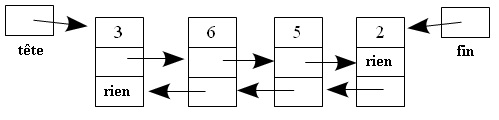
\includegraphics[width=13.203cm,height=3.175cm]{image/a2012Logique2eme-img008.png}
	\end{center}
	
	On peut facilement construire les classes ÉlémentListeBD et ListeBD 
	en adaptant légèrement les classes pour la liste
	chainée simple. La classe ListeBD aura comme attributs les deux accès 
	aux extrémités de la liste, nommés
	\textit{premier} et \textit{dernier}.
	
	\cadre{
		\begin{pseudo}
			\Class{ÉlémentListeBD<T>}
				\Private
					\Decl valeur~: T
					\Decl suivant~: ÉlémentListeBD<T>
					\Decl précédent~: ÉlémentListeBD<T>
				\Public
					\ConstrSign{ÉlémentListeBD<T>}{val~: T, suiv, prec~: ÉlémentListeBD<T>}
					\ConstrSign{ÉlémentListeBD<T>}{val~: T}
					\RComment précédent et suivant à rien
					\MethodSign{getvaleur}{}{T}
					\MethodSign{setValeur}{val~: T}{}
					\MethodSign{getSuivant}{}{ÉlémentListeBD<T>}
					\RComment ne renvoie rien si pas de suivant
					\MethodSign{setSuivant}{elt~: ÉlémentListeBD<T>}{}
					\MethodSign{getPrécédent}{}{ÉlémentListeBD<T>}
					\RComment ne renvoie rien si pas de précédent
					\MethodSign{setPrécédent}{elt~: ÉlémentListeBD<T>}{}
			\EndClass
		\end{pseudo}
	}
	
	\cadre{
		\begin{pseudo}
			\Class{ListeBD<T>}
				\Private
					\Decl premier~: ÉlémentListeBD<T>
					\Decl dernier~: ÉlémentListeBD<T>
				\Public
					\ConstrSign{ListeBD<T>}{}
					\MethodSign{getPremier}{}{ÉlémentListeBD<T>}
					\MethodSign{getDernier}{}{ÉlémentListeBD<T>}
					\MethodSign{estVide}{}{booléen}
					\MethodSign{insérerTête}{val~: T}{}
					\MethodSign{insérerFin}{val~: T}{}
					\MethodSign{insérerAprès}{elt~:	ÉlémentListeBD<T>, val~: T)}{}
					\MethodSign{insérerAvant}{elt~:	ÉlémentListeBD<T>, val~: T)}{}
					\MethodSign{supprimerTête}{}{}
					\MethodSign{supprimerFin}{}{}
					\MethodSign{supprimer}{elt~: ÉlémentListeBD<T>)}{}
			\EndClass
		\end{pseudo}
	}
	

%=========================
\section{Liste circulaire}
%=========================

	Dans une \textbf{liste circulaire}, le dernier élément ne référence 
	pas «~rien~» mais indique le premier élément.
	Schématiquement~:

	\begin{center}
	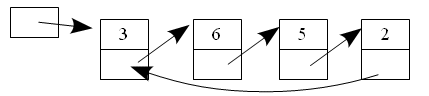
\includegraphics[width=11.351cm,height=2.54cm]{image/a2012Logique2eme-img009.png}
	\end{center}
	
	Il n'est pas nécessaire de créer une classe nouvelle pour les 
	éléments de la liste circulaire, puisqu'ils sont
	identiques à ceux d'une liste chainée simple. On peut faire fonctionner 
	ce type de liste avec les outils développés
	pour la liste chainée, il faut simplement veillez ici à la cohérence 
	de la liste circulaire, c'est-à-dire qu'à tout
	moment le dernier élément doit être lié au premier. Noter que premier 
	a ici un sens différent du point de vue logique,
	dans une liste circulaire il n'y a pas réellement de \textit{premier} 
	élément, mais un accès à un élément quelconque de
	la liste, peu importe sa position.
	
	
%==================
\section{Exercices}
%==================

	{\bfseries
	Remarques préliminaires}

	\begin{itemize}
		\item 
			\textit{Dans les exercices qui suivent, vous serez souvent amenés à 
			écrire des algorithmes similaires dont le code ne diffère
			qu'en un seul endroit. Dans cette situation, il faut toujours se 
			demander s'il n'est pas possible de factoriser le
			code, c'est-à-dire de le rendre modulaire de façon à limiter 
			l'écriture de code semblable.}
		\item
			\textit{Dans les exercices sur les listes, on s'efforcera toujours 
			de trouver la méthode la plus efficace (éviter de parcourir
			inutilement la liste) et aussi la plus économique (éviter si possible 
			les nouvelles demandes d'allocation d'éléments si
			ce n'est pas nécessaire).}
		\item 
			\textit{Sauf si c'est précisé, les exercices peuvent se faire 
			indifféremment en OO ou non, ce qui laisse la possibilité de
			s'entraîner dans les deux notations.}
	\end{itemize}
	
	\begin{Exercice}{Opérations de base}
		Écrire, dans la syntaxe de l'implémentation procédurale objet, 
		les modules qui correspondent aux méthodes de la liste 
		chainée dans la représentation OO, c'est-à-dire~:

		\begin{enumerate}
			\item {
				un module qui vérifie si une liste chainée est vide}
			\item {
				un module qui insère en début de liste un nouvel élément de valeur \textbf{val}}
			\item {
				un module qui insère un nouvel élément de valeur \textbf{val} après celui d'accès p}
			\item {
				un module qui supprime le premier élément d'une liste chainée}
			\item {
				un module qui supprime l'élément qui suit celui d'accès \textbf{p}}
		\end{enumerate}
	\end{Exercice}
	
	\begin{Exercice}{Insertions, recherches et suppressions}
		
		Soit une liste chainée contenant des valeurs d'un type T quelconque. Écrire~:

		\begin{enumerate}
			\item {
				un module qui ajoute dans la liste un nouvel élément de valeur 
				\textbf{val} (à l'endroit qui permet le code le plus simple)}
			\item {
				un module qui recherche dans la liste la valeur \textbf{val} 
				et retourne l'accès à l'élément qui le contient (ou rien si
				la valeur ne s'y trouve pas). Si la valeur s'y trouve plusieurs 
				fois, le module en retourne la première occurrence.}
			\item {
				un module qui retourne un booléen indiquant si la liste 
				contient la valeur \textbf{val}}
			\item {
				un module qui supprime de la liste le premier élément contenant 
				une valeur \textbf{val}. Le module retournera un booléen
				indiquant si la suppression a été réalisée~: vrai si \textbf{val} 
				a été supprimé, et faux sinon (parce que la valeur ne
				s'y trouvait pas).}
			\item {
				un module qui supprime de la liste toutes les occurrences de la valeur 
				\textbf{val} et retourne le nombre de suppressions réalisées}
		\end{enumerate}
		
		{\itshape
		N.B.~: cet exercice peut être réalisé de trois façons~(1) en procédural 
		(2) en orienté objet (3) sous forme de méthodes de la classe ListeChainée}
	\end{Exercice}

	\begin{Exercice}{Le grand nettoyage}
		Soit une liste chainée dont les valeurs (non ordonnées) sont des 
		entiers compris entre 1 et 10 inclus. On demande
		d'écrire l'algorithme qui supprime de cette liste toutes les 
		occurrences de la valeur la plus fréquente. En cas
		d'\textit{ex-æquo}, c'est la plus grande des valeurs qui est éliminée.

		\textit{Exemple}~: la liste (8, 7, 6, 7, 7, 1, 7, 1, 5, 7) devient (8, 6, 1, 1, 5).
	\end{Exercice}

	\begin{Exercice}{Liste chainée ordonnée}
		Soit une liste chainée dont les éléments sont triés (les 
		éléments sont d'un type T non précisé, mais on suppose que les
		opérateurs de comparaison (<, >, =,{\dots}) sont autorisés pour 
		ce type). Réécrire les modules de l'exercice 2 en effectuant 
		les changements optimisant le code et la performance.
	\end{Exercice}

	\begin{Exercice}{Pas de doublons}
		Soit une liste chainée dont les éléments sont triés (idem 
		que pour l'exercice précédent) mais \textbf{ne contenant pas
		de doublons}. Réécrire les modules de l'exercice 4 qui 
		nécessitent un changement ou une adaptation.
	\end{Exercice}

	\begin{Exercice}{Liste bidirectionnelle}
		Développer le code des méthodes introduites dans la classe ListeBD.
	\end{Exercice}
	
	\begin{Exercice}{Liste circulaire}
		Transformer la classe ListeChainée en ListeChainéeCirculaire, 
		en ne changeant que les méthodes qui nécessitent une
		adaptation. Ajouter dans cette classe une méthode qui calcule 
		la taille de la liste, et une méthode qui permet
		d'ajouter un élément de valeur donnée à l'emplacement qui 
		correspond au code le plus performant.
	\end{Exercice}

	\begin{Exercice}{Tassement de liste}
	
		Soit une liste chainée d'entiers dont les éléments sont ordonnés 
		en ordre croissant sur les valeurs, et dans laquelle
		plusieurs éléments consécutifs peuvent avoir la même valeur. 
		Écrire un algorithme qui supprime de cette liste toutes
		les valeurs redondantes.

		\textit{Exemple}~: la liste (5, 5, 7, 7, 7, 11, 13, 13, 15) devient (5, 7, 11, 13, 15)
	\end{Exercice}
	
	\begin{Exercice}{Inter-classement de listes}
		Soient deux listes chainées de même type d'éléments. On voudrait 
		créer à partir de celles-ci une liste chainée issue de
		l'inter-classement des éléments de ces deux listes, c'est-à-dire 
		contenant dans l'ordre le premier élément de la
		première liste, le premier élément de la seconde liste, 
		le 2\textsuperscript{ème} élément de la première liste, le
		2\textsuperscript{ème} élément de la seconde liste et ainsi de suite. 
		Si une des deux listes est plus longue, on
		rattache le reste de celle-ci à la fin de la liste obtenue par 
		l'inter-classement des premiers éléments.

		\textit{Exemple}~: l'inter-classement des listes (2, 5, 9, 8, 10) et 
		(7, 4, 3) donnera comme résultat la liste
		(2, 7, 5, 4, 9, 3, 8, 10)

		Réaliser cet exercice~:

		\begin{enumerate}
			\item {
				En créant une 3\textsuperscript{ème} liste 
				(les deux listes de départ restent intactes)}
			\item {
				Sans nouvelle demande d'allocation d'élément, c'est-à-dire 
				en incorporant les éléments de la 2\textsuperscript{ème}
				liste à la première.}
		\end{enumerate}
		
		N.B.~: \textit{si vous réalisez cet exercice en OO, vous aurez besoin 
		exceptionnellement d'une méthode } \textstyleCodeInsr{setPremier( )}
		\textit{ que nous n'avons pas introduite dans la classe ListeChainée, 
		son emploi étant assez rare.}
	\end{Exercice}
	
	\begin{Exercice}{Fusion de listes}
		Écrire un algorithme qui fusionne 2 listes chainées ordonnées 
		de même type d'éléments. Comme dans l'exercice précédent,
		on envisagera les cas ou (a) c'est une nouvelle liste qui 
		est créée (b) la seconde liste est incorporée à la première
		sans nouvelle demande d'allocation d'élément.
	\end{Exercice}
	
	\begin{Exercice}{Tri-fusion par éclatement des monotonies croissantes}
		Soit une liste chainée à valeurs entières. Une monotonie croissante 
		est une suite d'éléments qui se suivent et dont les
		valeurs sont dans l'ordre croissant. Le tri-fusion consiste à extraire 
		une monotonie, puis une autre, et ainsi de
		suite, et de fusionner chaque monotonie extraite avec le résultat 
		des fusions précédentes. Après la dernière fusion, la
		liste obtenue sera ordonnée, et la liste initiale aura donc été 
		transformée en une liste triée. Réaliser l'algorithme.
	\end{Exercice}

	\begin{Exercice}{Les ensembles}
		Définissons une classe Ensemble représentant un ensemble d'entiers 
		(au sens mathématique du terme). Développer le code
		des constructeurs et méthodes.

		\cadre{
			\begin{pseudo}
				\Class{Ensemble}
					\Private
						\Decl valeurs~: ListeChainée<entier>
						\RComment les valeurs seront ordonnées 
					\Public
						\ConstrSign{Ensemble}{}
						\LComment crée un ensemble vide 
						\MethodSign{ajoute}{val~: entier}{}
						\LComment ajoute une valeur à l'ensemble 
						\MethodSign{contient}{val~: entier}{booléen}
						\LComment indique si l'ensemble contient la valeur 
						\MethodSign{union}{autreEnsemble~: Ensemble}{Ensemble}
						\LComment crée l'ensemble contenant tous les éléments des 2 premiers 
						\MethodSign{intersection}{autreEnsemble~: Ensemble}{Ensemble}
						\LComment crée l'ensemble des éléments communs aux 2 premiers 
						\MethodSign{différence}{autreEnsemble~: Ensemble}{Ensemble}
						\LComment retourne l'ensemble des éléments qui ne sont pas dans le 2\textsuperscript{ème}ensemble 
				\EndClass
			\end{pseudo}
		}
	\end{Exercice}
	
	\begin{Exercice}{L'algorithme du survivant}
		Le jeu du survivant se déroule comme suit~: un nombre indéterminé de joueurs sont assis en cercle. Le meneur du jeu
		choisit un nombre entier au hasard (par ex. en lançant un dé) que nous appellerons le \textit{pas de décompte}.
		Ensuite, il parcourt le cercle de joueurs en tournant dans le sens horloger derrière eux tout en comptant une unité à
		chaque joueur rencontré, et ce jusqu'à ce que pas de décompte est atteint. Le joueur derrière lequel il s'arrête est
		alors éliminé, et le meneur recommence son décompte à partir du joueur restant suivant. Il recommence ceci jusqu'à ce
		qu'il ne reste plus qu'un seul joueur, qui est le «~survivant~» de ce jeu.

		Réaliser l'algorithme qui simule ce jeu. Les paramètres sont une liste chainée circulaire contenant les noms des
		joueurs, et le pas de décompte. On suppose que le premier élément auquel on accède dans la liste correspond au premier
		joueur compté par le meneur de jeu. L'algorithme retourne le nom du survivant.
	\end{Exercice}

	\begin{Exercice}{Polynôme}
	
		Vous vous rappelez, par votre cours de mathématique, 
		qu'un \textit{monôme} est une expression de la forme
		\textit{ax}\textit{n}, où \textit{a} 
		est le coefficient, \textit{x} la variable et \textit{n}
		l'exposant (ex.~: $3x^2$). Un \textit{polynôme} est alors 
		une somme de monômes (ex.~: $3x^4-x^2+2$)

		\textit{Représentation}~: convenons de représenter un monôme 
		comme une simple structure avec 2 champs~: le coefficient
		et l'exposant. Un polynôme sera alors représenté comme une 
		liste chainée de monômes triés en ordre décroissant sur
		l'exposant.

		\textit{Problème}~: écrire un module permettant d'additionner 2 polynômes 
		et un autre permettant de les soustraire.
	\end{Exercice}

	\begin{Exercice}{Matrice creuse}
		Une matrice creuse est une matrice où la plupart des éléments sont nuls. 
		On les rencontre beaucoup dans des problèmes
		physiques impliquant des systèmes linéaires. Représenter une telle 
		matrice par un tableau classique à 2 dimensions
		n'est efficace ni en terme d'espace mémoire (une matrice 
		1000 \textsf{x} 1000 va contenir un million de valeurs presque
		toutes nulles) ni en terme de temps de calcul (beaucoup de calculs 
		avec des 0). C'est pourquoi on utilise souvent dans
		ce cas là un maillage de listes (une liste par ligne et une liste 
		par colonne).

		\textit{Exemple}~: La matrice~:

		\begin{figure}
			\centering
			\begin{minipage}{2.388cm}
			\begin{flushleft}
			\tablefirsthead{}
			\tablehead{}
			\tabletail{}
			\tablelasttail{}
			\begin{supertabular}{|m{0.393cm}|m{0.393cm}|m{0.393cm}|m{0.41000003cm}|}
			\hline
			{ 4} &
			{ 0} &
			{ 0} &
			{ 7}\\
			\hline
			{ 0} &
			{ 9} &
			{ 0} &
			{ 0}\\
			\hline
			{ 0} &
			{ 0} &
			{ 0} &
			{ 2}\\
			\hline
			\end{supertabular}
			\end{flushleft}
			\end{minipage}
		\end{figure}
		
		\bigskip
		
		\bigskip
		
		\bigskip
		
		sera représentée comme le suggère le schéma suivant~:

		\begin{center}
		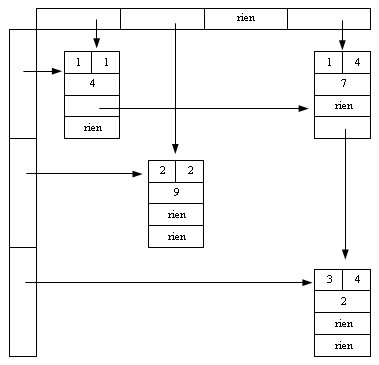
\includegraphics[width=10.028cm,height=9.657cm]{image/a2012Logique2eme-img010.png}
		\end{center}
		
		Chaque élément de la liste contient le numéro de ligne et 
		de colonne, la valeur, un lien vers l'élément non nul suivant
		dans la ligne et un lien vers l'élément non nul suivant dans 
		la colonne. On dispose également d'un tableau pour les
		têtes de lignes et un tableau pour les têtes de colonnes.

		On vous demande de~:

		\begin{enumerate}
			\item 
				Définir les attributs de la classe ÉlémentMatriceCreuse représentant un élément de la matrice.
			\item 
				Définir les attributs de la classe MatriceCreuse ainsi que
		
				\cadre{
					\begin{pseudo}
						\ConstrSign{MatriceCreuse}{nbLignes, nbColonnes~: entiers}
						\LComment construit une matrice vide
						\MethodSign{get}{ligne, col~: entiers}{entier}
						\LComment donne la valeur de l'élément de la matrice en position (ligne, col)
						\MethodSign{set}{ligne, col, valeur~: entiers}{}
						\LComment affecte une valeur à l'élément de la matrice en position (ligne, col);
						\LComment si la valeur est nulle il faudra peut-être supprimer un élément;
						\LComment au contraire, si la valeur est non nulle, il faudra peut-être en ajouter.
					\end{pseudo}
				}
		\end{enumerate}
	\end{Exercice}

